\chapter{Shared Memory Architectures}
\label{ch:04/shared-memory-architectures}

Shared Memory Architectures are a type of MIMD architecture where all processors share the same memory space, and can access it directly. This is the most common architecture for multi-core processors (\textit{``multiprocessors''}).

They mirror the Von Neumann architecture, with multiple processors sharing the same memory space.

\section{Von Neumann Bottleneck}

\begin{definition}[von Neumann Bottleneck]
   The \textit{von Neumann bottleneck} is a limitation on throughput caused by the standard personal computer architecture. The term is named for John von Neumann, who is credited with developing the von Neumann architecture, in which programs and data are stored in the same memory. \ul{The bottleneck refers to the limited data transfer rate between a computer's CPU and memory compared to the amount of memory.}
\end{definition}

\begin{figure}[htbp]
   \centering
   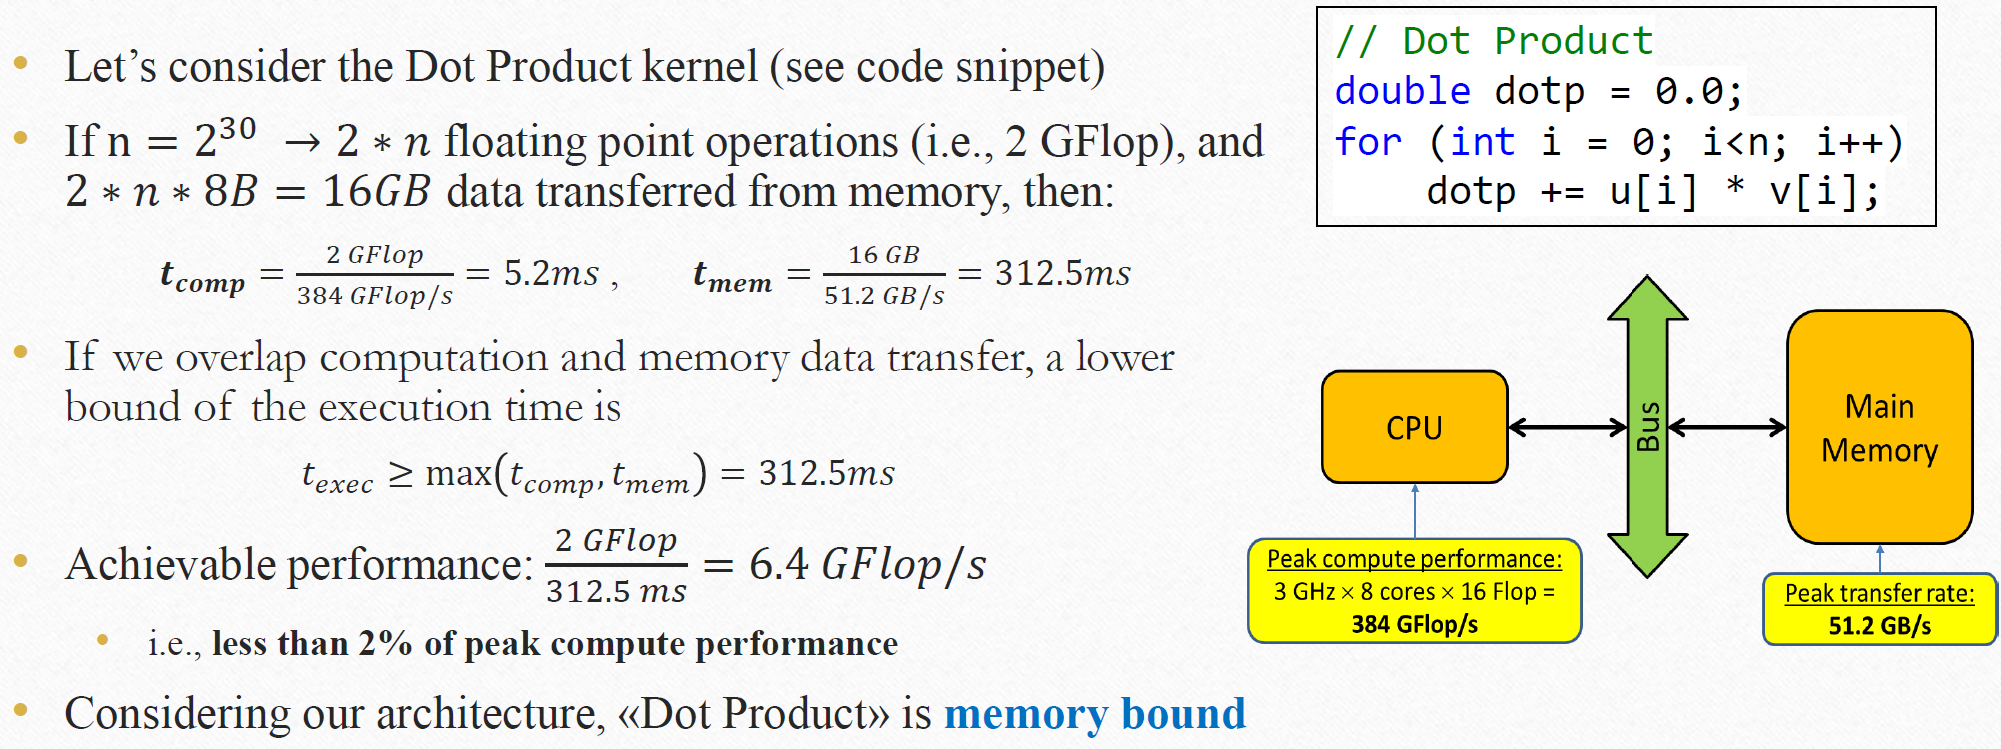
\includegraphics{images/04/neumann_example.png}
   \caption{von Neumann Bottleneck example}
   \label{fig:04/neumann_example}
\end{figure}

In the example in Figure \ref{fig:04/neumann_example}, the CPU is waiting for the data to be loaded from memory, which is a slow operation, leading to \ul{exploiting only the 2\% of the CPU capabilities.}

\subsection{Caches}

\begin{paracol}{2}
   Back in the day, the solution was to \textit{``move the data closer to the CPU''}, introducing \textbf{memory hierarchy} and \textbf{caches}.

   Usally, L1 and L2 are private to each core, while L3 is shared among all cores.
   \switchcolumn
   
   \begin{figure}[htbp]
      \centering
      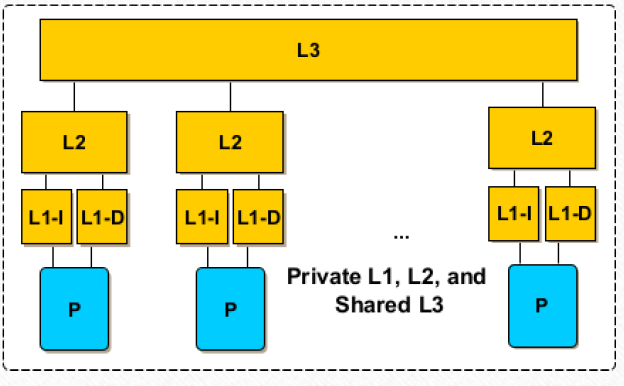
\includegraphics{images/04/caches_hierarchy.png}
      \caption{Caches hierarchy}
      \label{fig:04/caches_hierarchy}
   \end{figure}
\end{paracol}

If a matrix of the previous example in Fig. \ref{fig:04/neumann_example} is entirely stored in cache, then the achievable performance is \ul{223 GFLOPS, which is about 60\% of the peak power.}

If the matrices do not fit in the cache, the performance drops since we need to trap to the main memory to fetch missing data.\\
So, the problem shifts to understand how to exploit the cache to its fullest.

\section{Locality Principle}

The locality principle is the driving force that makes the cache work. Locality increases the probability of reusing data blocks that were previously moved from level $n$ to level $n-1$.
\begin{itemize}
   \item \textbf{Temporal Locality}: if a data is accessed, it is likely to be accessed again soon.
   \note{Cache mapping strategy (Direct/associative) and the replacement policy (LRU, FIFO, Random etc.) are crucial to exploit temporal locality.}
   \item \textbf{Spatial Locality}: if a data is accessed, it is likely that nearby data will be accessed soon.
\end{itemize}

\subsection{Measuring CPU time with caches}
\begin{equation}
   CPU_{time} = ClockCycles \cdot ClockCycleTime = IC \cdot ClockCycleTime
\end{equation}
\begin{itemize}
   \item IC: Instruction Count (number of instructions executed)
   \begin{itemize}
      \item $IC = IC_{CPU} + IC_{MEM}$
   \end{itemize}
   \item CPI: Cycles Per Instruction
   \begin{itemize}
      \item $CPI = \dfrac{ClockCycles}{IC}$
      \item $CPI = \dfrac{IC_{CPU}}{IC} \cdot CPI_{CPU} + \dfrac{IC_{MEM}}{IC} \cdot CPI_{MEM}$ where $CPI_{CPU}$ are the average cycles per ALU instruction and $CPI_{MEM}$ are the average cycles per memory instruction.
      \item Considering that each memory instruction may generate a cache hit or miss with a given probability, and naming $HitRate$ the probability of a cache hit, we can write 
      \begin{equation}
         CPI_{MEM} = HitRate \cdot CPI_{MEM - Hit} + (1-HitRate) \cdot CPI_{MEM - Miss}
      \end{equation}
   \end{itemize}
\end{itemize} 

\subsection{Cache Algorithms}
\begin{enumerate}
   \item \textit{What do we load from main memory?}
   \item \textit{Where do we store it in the cache?}
   \item \textit{Cache is full, what should we evict?}
\end{enumerate}

\note{At the beginning of the second half of the $4^{th}$ lecture, the professor displays how to VPN in the unipi and then ssh to the servers.}

\subsection{Cache mapping and eviction strategies}
\begin{itemize}
   \item \textbf{Direct-mapped} cache: each memory block can be placed in only one cache line.
   \item \textbf{n-way} set associative cache: each memory block can be placed in $n$ cache lines.
   \item \textbf{Least Recently Used} (LRU) cache: the block that has been accessed the least recently is evicted.
\end{itemize}

\framedt{Transposing Matrices}{
   Suppose you have to multiply matrix A and B. If you access A as rows, you'll access B as columns.\\
   Since matrices are stored in row-major order, you won't exploit spatial locality on B, and for each element of A you'll have a cache miss on B, creating the need to evict a line and load another one in cache.\\
   \textbf{Transposing} B would solve the problem, since you would access B as rows, exploiting spatial locality.

   Prof. Torquati displayed that transposing and then multiplying the matrices would lead to a 2x speedup.
   \note{17s vs 37s}
}

\subsection{Cache Write Policies}
Data in cache may be inconsistent with the value in memory, leading to the need to write back the data to memory. There are two policies:
\begin{itemize}
   \item \textbf{Write-through}: data is written to both cache and memory. It is simple but slow.
   \item \textbf{Write-back}: data is written only to the cache, and then to memory when the block is evicted. It is faster but more complex.
   \begin{itemize}
      \item Caches mark data in the cache as dirty (Dirty bit)
      \item When a dirty line is evicted, it is written in main memory
      \item A store write buffer is generally used to reduce the cost of cache writes
   \end{itemize}
\end{itemize}

\subsection{Cache Coherence}
\begin{paracol}{2}
   With private caches per core, it is possible to have several copies of shared data in distinct caches, each cache stores a different value for a single address location.
   
   \begin{definition}[Cache incosistency]
      Two caches store different values for the same variable.
   \end{definition}
   
   \switchcolumn

   \begin{figure}[htbp]
      \centering
      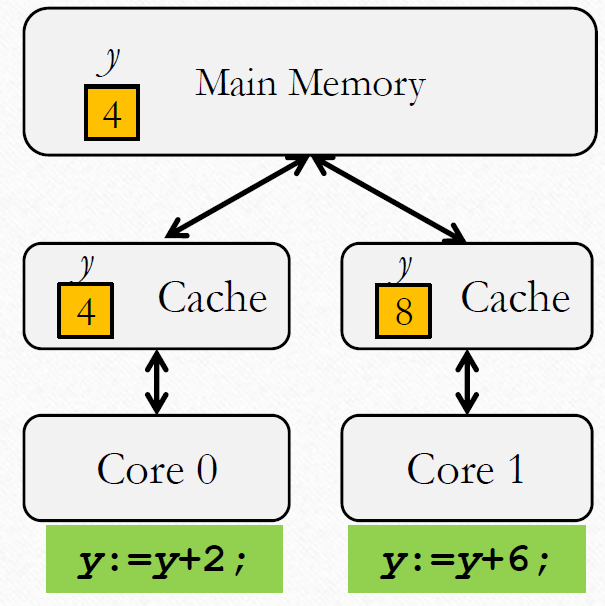
\includegraphics{images/04/cache_coherence.png}
      \caption{Cache incosistency problem}
      \label{fig:04/cache_coherence}
   \end{figure}

\end{paracol}

Hardware firmware automatically solves this problem, but it is important to know that it exists.
The algorithms responsible for this are called \textbf{cache coherence protocols}, a famous one is the \textbf{MESI} protocol, but we ain't going to study it.
Note however that \ul{the cache coherence protocol granularity is the \textit{cache line}, not the \textit{single variable}.}
   
\section{Suggested readings}
\begin{itemize}
   \item
      Chapter 3.1 of the Parallel Programming Concept and Practice book
   \item
      Cache-coherence protocols: ``A Primer on Memory Consistency and Cache Coherence'' Daniel J. Sorin, Mark D. Hill, and David A. Wood
\end{itemize}